\section{\ac{AI} in software development}
  Artificial intelligence is rapidly becoming part of everyday software engineering practice. What only a few years ago looked experimental is now increasingly presented as ordinary development tooling. Coding assistants, chat-based code generation, automated review systems, and agent-based tools are no longer discussed only as research prototypes, but as products that are actively being integrated into professional workflows \cite{AI2024Stack,staffSurveyAIWave2024,DORAAccelerateState}.

  For this reason I deem it highly valuable to research these \ac{AI} tools to get to know them, how they work and what they bring to the table. Not knowing what the strengths and weaknesses of \ac{AI} use in software development and not knowing how to use them effectively will be a serious disadvantage in the working life seeing as it is being adopted so rapidly.

  \subsection{Increasing adoption}
  Several recent surveys suggest that \ac{AI} tools are already widespread among developers. While the exact percentages vary depending on the survey population and the wording of the question, the overall trend is consistent: developers are using these tools, organizations are investing in them, and their role in the development workflow is growing \cite{AI2024Stack,staffSurveyAIWave2024,DORAAccelerateState}. Figure~\ref{fig:ai_dev_adoption} summarizes a few representative results from widely cited industry reports. The exact numbers should not be treated as directly comparable, since the surveys ask slightly different questions, but together they illustrate that \ac{AI}-assisted development has moved well beyond early experimentation.

  In practical terms, this means that \ac{AI} is increasingly becoming part of the normal tooling landscape of software engineering, much like version control, testing frameworks, or static analysis tools. It is therefore reasonable for a thesis about software development to treat \ac{AI} not as a novelty, but as a serious development aid that deserves explicit reflection \cite{staffSurveyAIWave2024,DORAAccelerateState}.

  \begin{figure}[htbp]
  \centering
  \resizebox{0.92\textwidth}{!}{%
  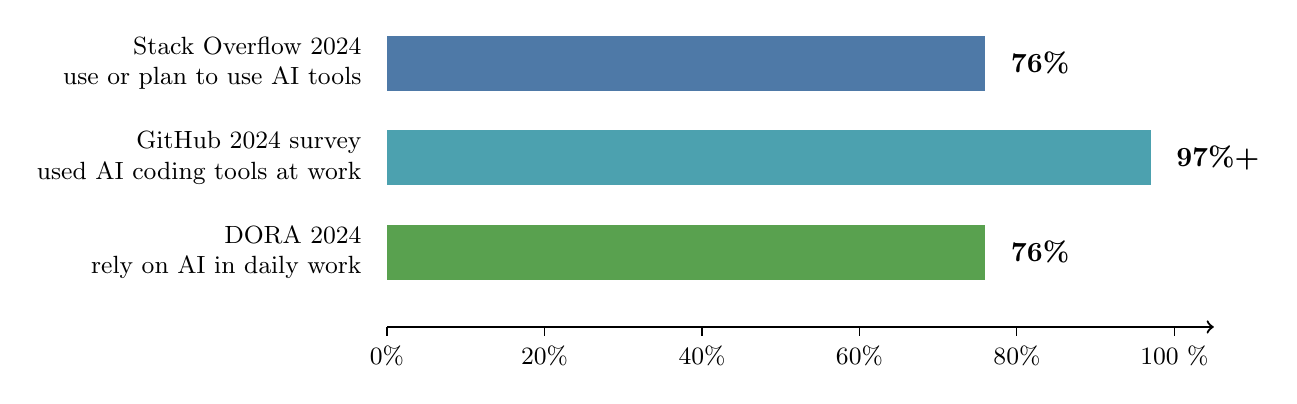
\begin{tikzpicture}[font=\small]
    \definecolor{adoptblue}{RGB}{78,121,167}
    \definecolor{adoptteal}{RGB}{76,161,175}
    \definecolor{adoptgreen}{RGB}{89,161,79}

    \draw[->, thick] (0,0) -- (10.5,0);

    \foreach \x/\label in {
      0/0,
      2/20,
      4/40,
      6/60,
      8/80,
      10/100
    }{
      \draw (\x,0) -- (\x,-0.12);
      \node[below] at (\x,-0.12) {\label\%};
    }

    \fill[adoptblue] (0,3.0) rectangle (7.6,3.7);
    \fill[adoptteal] (0,1.8) rectangle (9.7,2.5);
    \fill[adoptgreen] (0,0.6) rectangle (7.6,1.3);

    \node[anchor=east, align=right] at (-0.2,3.35) {Stack Overflow 2024\\use or plan to use AI tools};
    \node[anchor=east, align=right] at (-0.2,2.15) {GitHub 2024 survey\\used AI coding tools at work};
    \node[anchor=east, align=right] at (-0.2,0.95) {DORA 2024\\rely on AI in daily work};

    \node[anchor=west, font=\bfseries] at (7.8,3.35) {76\%};
    \node[anchor=west, font=\bfseries] at (9.9,2.15) {97\%+};
    \node[anchor=west, font=\bfseries] at (7.8,0.95) {76\%};
  \end{tikzpicture}%
  }
  \caption{Selected survey results illustrating the prevalence of \ac{AI}-assisted software development. The figures are based on different populations and question formulations, so they should be read as trend indicators rather than directly comparable measurements.}
  \label{fig:ai_dev_adoption}
\end{figure}


  \subsection{Potential benefits}
  One important reason for the rapid adoption of \ac{AI} tools is that they appear to offer real gains in productivity and workflow support. These gains do not necessarily mean that the model replaces the developer. Rather, the benefit often lies in assisting with time-consuming or repetitive tasks such as code completion, boilerplate generation, refactoring suggestions, test drafting, documentation support, and codebase exploration. This can allow the developer to spend a greater proportion of time on design decisions, debugging strategy, and evaluation of alternative solutions.

  Recent empirical work also suggests that these benefits are not only anecdotal. Controlled and field-based studies indicate that access to coding assistants can increase the rate at which software tasks are completed, although the size of the effect depends on context, task type, and developer experience \cite{cuiEffectsGenerativeAI2025}. At the same time, many studies and reports frame the benefit less as fully autonomous programming and more as augmented development, where the developer remains responsible for understanding and validating the result \cite{staffSurveyRevealsAIs2023,CodexAICoding,CodexNowGenerally2026}.

  \subsection{Limitations}
  At the same time, increased adoption does not imply unconditional trust. One of the clearest themes in recent literature and survey material is that developers often find \ac{AI} useful while still being skeptical of its output \cite{AI2024Stack,wangInvestigatingDesigningTrust2023}. This skepticism is well justified. \ac{AI}-generated code may be syntactically correct while still misunderstanding requirements, introducing subtle bugs, using poor abstractions, or suggesting insecure solutions. It can also create the false impression that a difficult problem has been solved simply because a fluent-looking answer has been produced.

  For this reason, the value of \ac{AI} in software development depends heavily on verification, domain understanding, and responsible use. A developer who relies on \ac{AI} without understanding the surrounding system risks turning the tool into a crutch. By contrast, a developer who already understands the problem domain can use \ac{AI} more effectively as an assistant: to accelerate drafting, explore alternatives, and reduce routine effort while still retaining control of the technical decisions \cite{wangInvestigatingDesigningTrust2023}.

  This perspective aligns well with the idea of appropriate trust. The goal is not to reject \ac{AI}, but to use it with enough understanding that its contributions can be evaluated critically. In other words, \ac{AI} can improve development speed and convenience, but only if the human developer remains responsible for interpretation, validation, and final judgment \cite{AI2024Stack,wangInvestigatingDesigningTrust2023,DORAAccelerateState}.

  \subsection{Relevance to this thesis}
  In this thesis, \ac{AI} is not treated as a replacement for software engineering work, but as a tool that may support the development process. This is the reason the first two iterations were developed without \ac{AI} assistance. Doing the early work manually helped establish a basic understanding of the musical domain, the program structure, and the design trade-offs involved in the project. Without that foundation, it would be much harder to judge whether \ac{AI}-generated suggestions were correct, useful, or aligned with the goals of the system.

  The third iteration therefore uses \ac{AI} in a more deliberate way. By that stage, the project has already accumulated enough structure and domain knowledge that \ac{AI} can be used more productively as a development aid. This makes it possible to evaluate not only whether the final system improves, but also whether \ac{AI} is practically useful in a constrained, iterative, technically demanding development process. The aim is thus not to let \ac{AI} carry the work, but to investigate whether it can function as a tool for assisting and streamlining the work.
